% -*- latex -*-
%%%%%%%%%%%%%%%%%%%%%%%%%%%%%%%%%%%%%%%%%%%%%%%%%%%%%%%%%%%%%%%%
%%%%%%%%%%%%%%%%%%%%%%%%%%%%%%%%%%%%%%%%%%%%%%%%%%%%%%%%%%%%%%%%
%%%%
%%%% This text file is part of the source of 
%%%% `The Art of HPC, vol 1: The Science of Computing'
%%%% by Victor Eijkhout, copyright 2012-2023
%%%%
%%%% This book is distributed under a Creative Commons Attribution 3.0
%%%% Unported (CC BY 3.0) license and made possible by funding from
%%%% The Saylor Foundation \url{http://www.saylor.org}.
%%%%
%%%% graphalgorithms.tex : application chapter; there is also a tutorial
%%%%
%%%%%%%%%%%%%%%%%%%%%%%%%%%%%%%%%%%%%%%%%%%%%%%%%%%%%%%%%%%%%%%%
%%%%%%%%%%%%%%%%%%%%%%%%%%%%%%%%%%%%%%%%%%%%%%%%%%%%%%%%%%%%%%%%
\label{sec:graph-analytics}

Various problems in scientific computing can be formulated as graph
problems;
for an introduction to graph theory see Appendix~\ref{app:graph}).
For instance, you have 
encountered the problems of load
balancing (section~\ref{sec:graph-loadbalancing}) and finding
independent sets (section~\ref{sec:redblackgreen}).

Many traditional graph algorithms are
not immediately, or at least not efficiently, applicable, since the
graphs are often distributed, and traditional graph theory assumes global
knowledge of the whole graph. Moreover, graph theory is often concerned
with finding the optimal algorithm, which is usually not a parallel one.
Conversely, in parallel we may get enough of a speedup that we
can afford to waste some cycles on an algorithms that is not optimal sequentially.
Therefore, parallel graph algorithms are a field of study by themselves.

Recently, new types of graph computations in have arisen in scientific
computing. Here the graph are no longer tools, but objects of study
themselves. Examples are the \indexterm{World Wide Web} or the
\indextermsub{social}{graph} of \indexterm{Facebook}, or the graph
of all possible \indexterm{protein interactions} in a living organism.

For this reason, combinatorial computational
science is becoming a discipline in its own right.
In this section we look at \indextermbus{graph}{analytics}:
computations on large graphs. We start by discussing some classic
algorithms, but we give them in an algebraic framework that will
make parallel implementation much easier.

\Level 0 {Traditional graph algorithms}
\label{sec:graph-alg}

We start by looking at a few `classic' graph algorithms, and we
discuss how they can be implemented in parallel. The connection
between graphs and sparse matrices (see Appendix~\ref{app:graph}) will
be crucial here: many graph algorithms have the structure of
a \emph{sparse matrix-vector
multiplication}\index{sparse!matrix-vector product!in graph theory}.

\Level 1 {Shortest path algorithms}
\label{sec:sssp}

There are several types of shortest path algorithms. For instance,
in the \indextermsub{single source}{shortest path} algorithm
one wants the shortest path from a given node to any other node.
In \indextermsub{all-pairs}{shortest path} algorithms
one wants to know the shortest distance between any two nodes.
Computing the actual paths is not part of these algorithms; 
however, it is usually easy to include some information by
which the path can be reconstructed later.

We start with a simple algorithm: finding the single source shortest
paths in an unweighted graph. This is simple to do with a \acf{BFS}:
in each step we have a set~$U$ of nodes for which the shortest distances
are known, and we consider the set~$V$ of their neighbors.

\begin{displayalgorithm}
  \Input{A graph, and a starting node~$s$}
  \Output{A function $d(v)$ that measures the distance from $s$ to~$v$}
  Let $s$ be given, and set $d(s)=0$\;
  Initialize the finished set as $U=\{s\}$\;
  Set $c=1$\;
  \While{not finished}{
    Let $V$ be the set of neighbours of $U$ that are not themselves in $U$\;
    \If{$V=\emptyset$}{We're done}\Else{
      \For{$v\in V$}{Set $d(v)=c+1$}
    $U\leftarrow U\cup V$\;
    Increase $c\leftarrow c+1$
    }
  }
\end{displayalgorithm}

This way of formulating an algorithm is useful for theoretical purposes:
typically you can formulate a \indexterm{predicate} that is true
for every iteration of the while loop. This then allows you to prove
that the algorithm terminates and that it computes what you intended it to compute.
And on a traditional processor this would indeed be how you program 
a graph algorithm. However, these days graphs such as from Facebook 
can be enormous, and you want to program your graph algorithm in
parallel.

In that case, the traditional formulations fall short:
\begin{itemize}
\item They are often based on queues to which nodes are added or subtracted; this means
  that there is some form of shared memory.
\item Statements about nodes and neighbours are made without wondering if these
  satisfy any sort of spatial locality; if a node is touched more than once there is
  no guarantee of temporal locality.
\end{itemize}

\Level 1 {Floyd-Warshall all-pairs shortest path}
\label{sec:floyd}
\index{Floyd-Warshall algorithm|(}

The \emph{Floyd-Warshall algorithm} is an example of an all-pairs
shortest paths algorithm. It is a \indexterm{dynamic programming}
algorithm that is based on gradually increasing the set of intermediate
nodes for the paths.
Specifically,  in step~$k$ all paths $u\rightsquigarrow v$ are considered 
that have intermediate nodes in the set $k=\{0,\ldots,k-1\}$, and $\Delta_k(u,v)$ 
is the defined as the path length from $u$ to~$v$ where all intermediate nodes
are in~$k$.
Initially, for $k=0$ this means that there are no intermeidate edges,
so only graph edges are considered;
when $k\equiv |V|$ we have considered all possible paths and we are done.

The computational step is
\begin{equation}
  \Delta_{k+1}(u,v) = \min\bigl\{ \Delta_k(u,v),
  \Delta_k(u,k)+\Delta_k(k,v) \bigr\}.
  \label{eq:floyd-allpairs}
\end{equation}
that is, the $k$-th estimate for the distance $\Delta(u,v)$ is the minimum
of the old one, and a new path that has become feasible now that we
are considering node~$k$. This latter path is found by
concatenating paths $u\rightsquigarrow k$
and~$k\rightsquigarrow\nobreak v$.

Writing it algorithmically:
\begin{displayalgorithm}
  \For {$k$ from zero to $|V|$}{
      \For {all nodes $u,v$} {
        $\Delta_{uv} \leftarrow f(\Delta_{uv},\Delta_{uk},\Delta_{kv})$
      }
  }
\end{displayalgorithm}
we see that this algorithm has a similar structure to Gaussian elimination, 
except that there the inner loop would be `for all $u,v>k$'.
(One could also compare this to the \indextermbus{Gauss}{Jordan} algorithm.)

Algebraically:
\begin{displayalgorithm}
  \For {$k$ from zero to $|V|$} {
    $D\leftarrow D._{\min} \bigl[D(:,k) \mathbin{\min\cdot_+} D(k,:)  \bigr]$
  }
\end{displayalgorithm}

The Floyd-Warshall algorithm does not tell you the actual
path. Storing those paths during the distance calculation above is
costly, both in time and memory. A~simpler solution is possible: we
store a second matrix~$n(i,j)$ that has the highest node number of the
path between $i$ and~$j$.

\begin{exercise}
  Include the calculation of $n(i,j)$ in the Floyd-Warshall algorithm,
  and describe how to use this to find the shortest path between $i$
  and~$j$ once $d(\cdot,\cdot)$ and $n(\cdot,\cdot)$ are known.
\end{exercise}

In section~\ref{sec:fill} you saw that the factorization of sparse
matrices leads to \emph{fill-in}\index{fill-in!in graph algorithms},
so the same problem occurs here. This requires flexible data structures,
and this problem becomes even worse in parallel; see section~\ref{sec:random-graph-product}.

\index{Floyd-Warshall algorithm|)}

\Level 1 {Spanning trees}
\label{sec:dijkstra}

In an undirected graph $G=\langle V,E\rangle$, we call $T\subset E$ a~`tree'
if it is connected and acyclic. It is called a \indexterm{spanning tree}
if additionally its edges contain all vertices.
If the graph has edge weights
$w_i\colon i\in E$, the tree has weight $\sum_{e\in T} w_e$, and
we call a tree a \indextermbus{minimum}{spanning tree} if it has minimum weight.
A~minimum spanning tree need not be unique.

\indexterm{Prim's algorithm}, a slight variant of
\indexterm{Dijkstra's shortest path algorithm}, computes a spanning
tree starting at a root. The root has path length zero, and all other
nodes have path length infinity.
In each step, all nodes connected to the known tree
nodes are considered, and their best known path length updated.

\begin{displayalgorithm}
  \Input{A graph $\langle V,E\rangle$ and node $s\in V$}
  \Output{A function $\ell(\cdot)$ giving the shortest distance of any node to~$s$}
  \For {all vertices $v$}{$\ell(v)\leftarrow\infty$}
  $\ell(s)\leftarrow 0$\;
  $Q\leftarrow V-\{s\}$ and $T\leftarrow \{s\}$\;
  \While{$Q\not=\emptyset$} {
    let $u$ be the element in $Q$ with minimal $\ell(u)$ value\;
    remove $u$ from $Q$, and add it to $T$\;
    \For {$v\in Q$ with $(u,v)\in E$} {
      \If {$\ell(u)+w_{uv}<\ell(v)$} {Set $\ell(v)\leftarrow \ell(u)+w_{uv}$}
    }
  }
\end{displayalgorithm}

\begin{figure}[ht]
  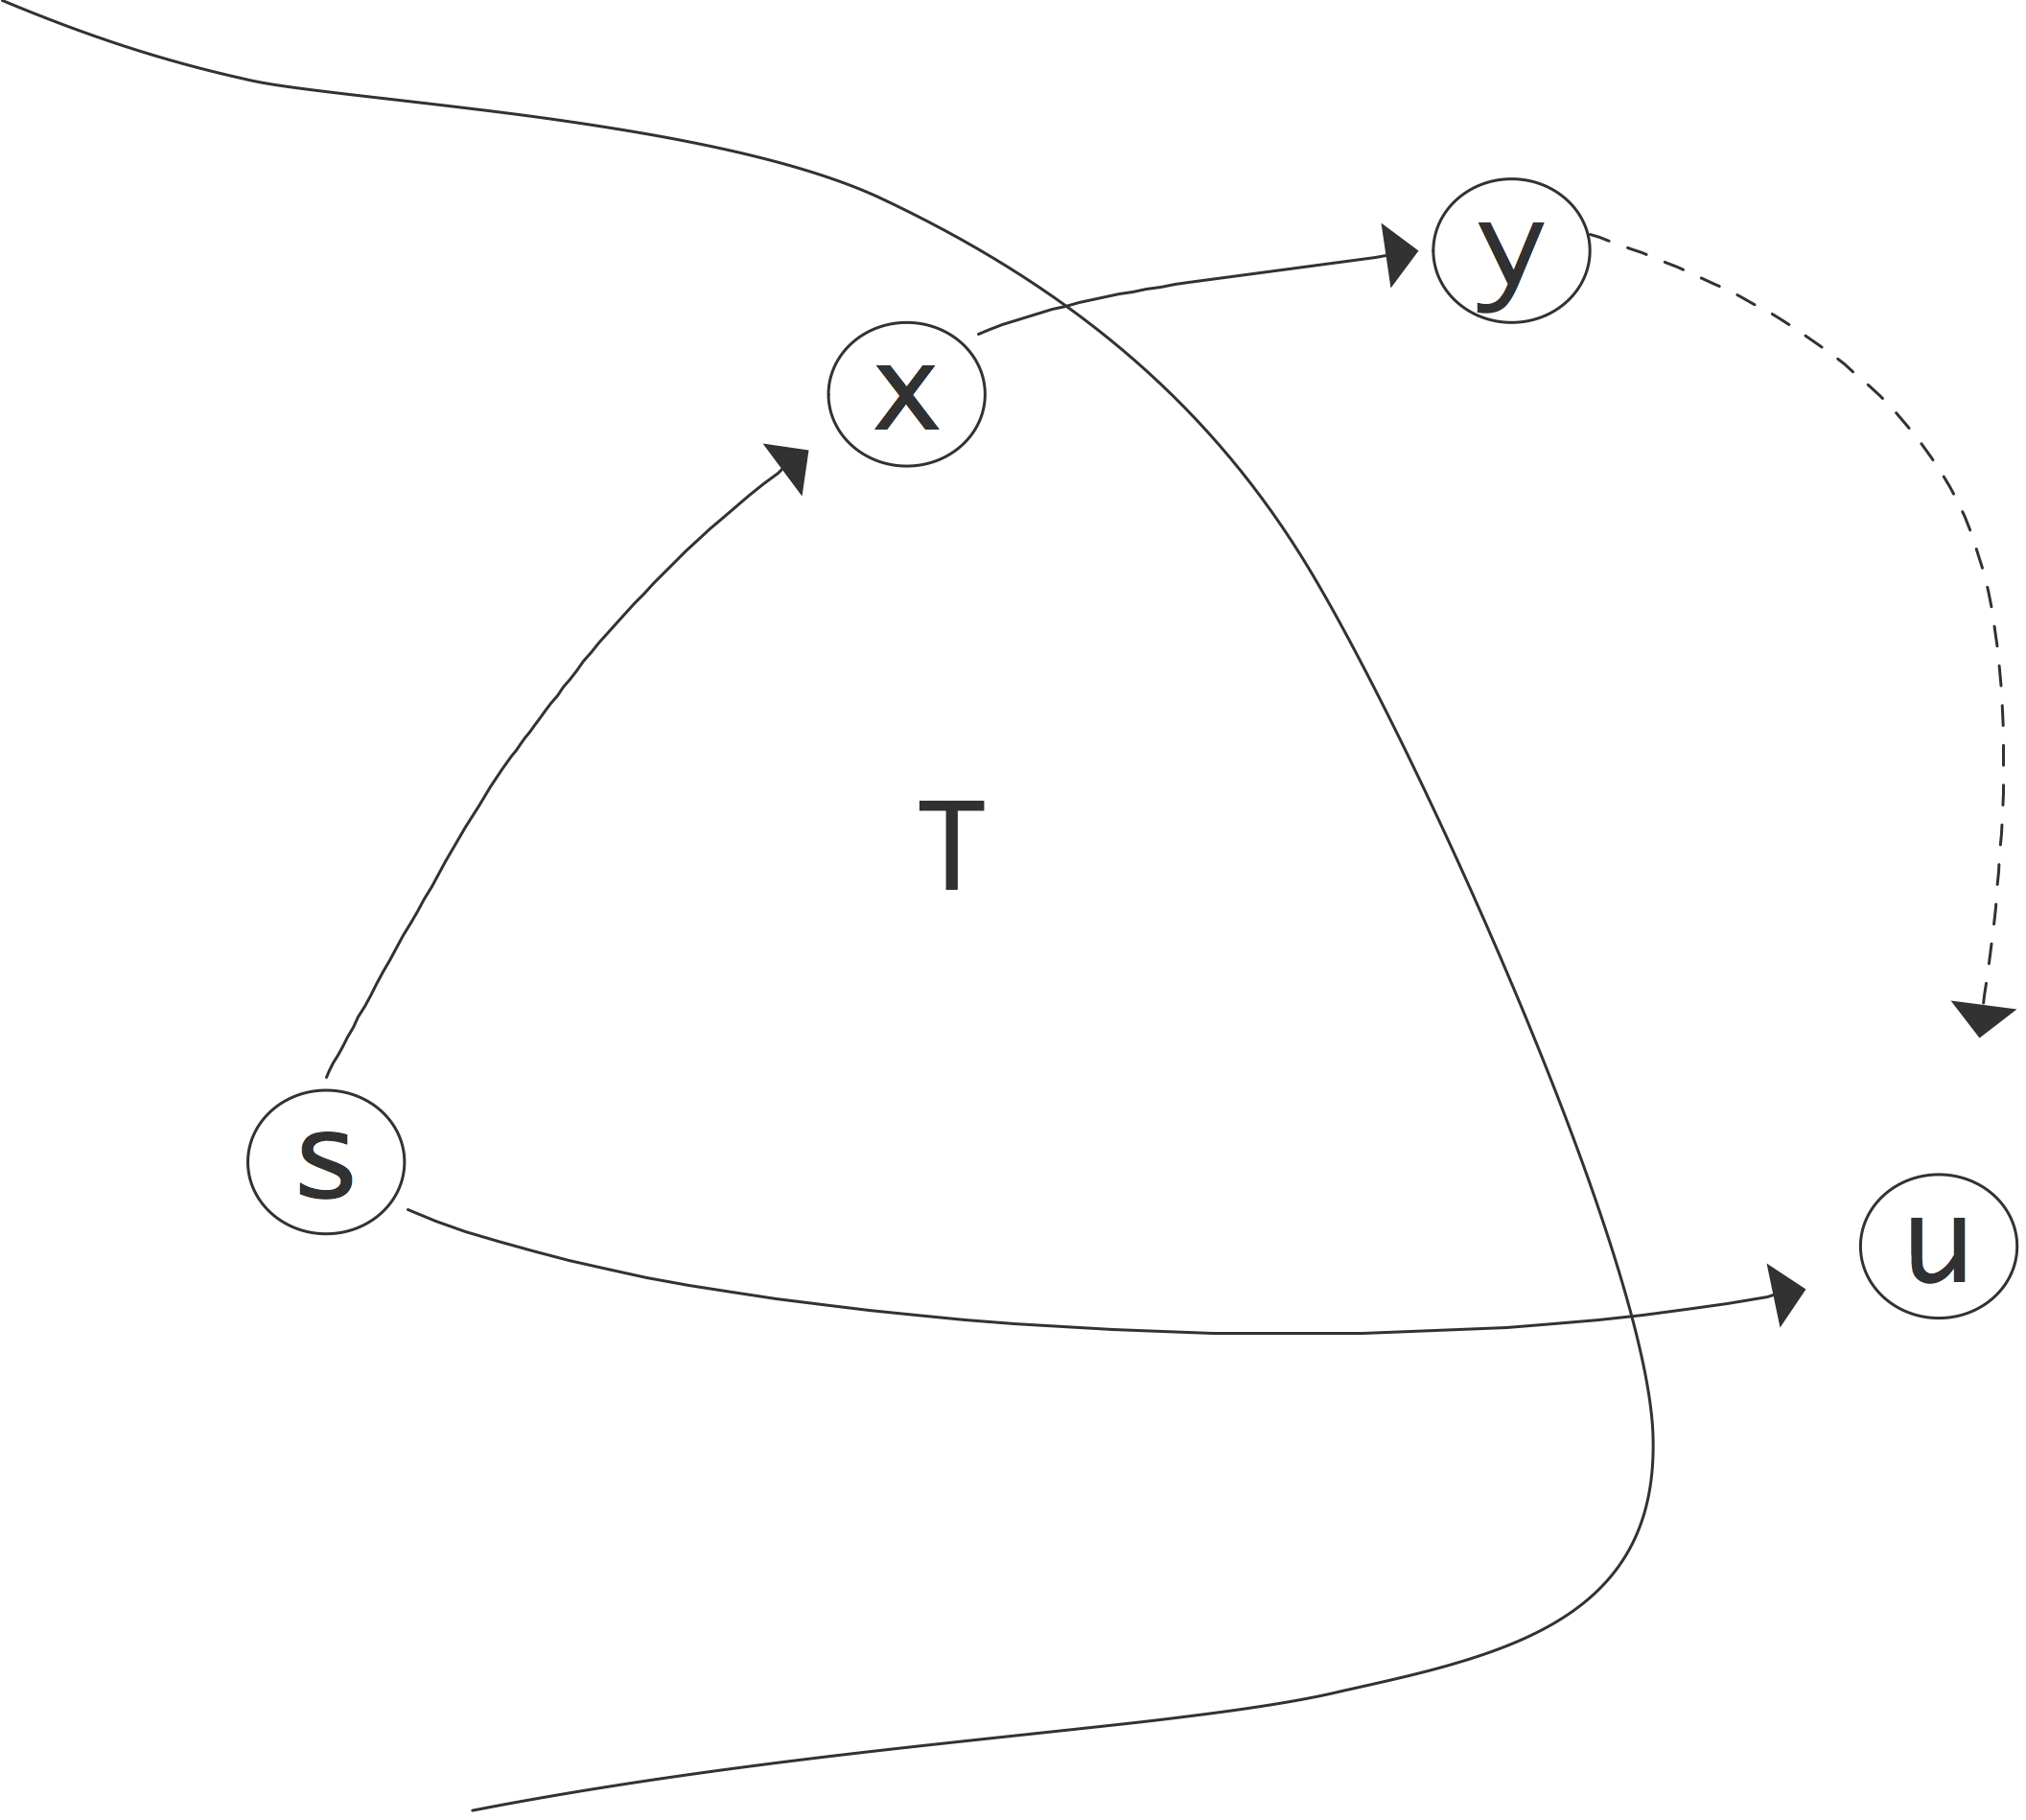
\includegraphics[scale=.12]{dijkstra-proof}
  \caption{Illustration of the correctness of Dijkstra's algorithm.}
  \label{fig:dijkstra-proof}
\end{figure}

\begin{theorem}
  The above algorithm computes the shortest distance from each
  node to the root node.
\end{theorem}
\begin{proof}
  The key to the correctness of this algorithm is the fact that
  we choose~$u$ to have minimal $\ell(u)$ value. Call the true shortest path
  length to a vertex~$L(v)$. Since we start with an $\ell$~value of infinity and
  only ever decrease it, we always have $L(v)\leq\ell(v)$.

  Our induction hypothesis will be that, at any stage in the algorithm,
  for the nodes in the current~$T$ the path length is determined correctly:
  \[ u\in T\Rightarrow L(u)=\ell(u). \]
  This is certainly true when the tree consists only of the root~$s$.
  Now we need to prove the induction step: if for all nodes in the
  current tree the path length is correct, then we will also 
  have $L(u)=\ell(u)$. 

  Suppose this is not true, and there is another path that is shorter.
  This path needs to go through some node~$y$ that is not currently in~$T$;
  this illustrated in figure~\ref{fig:dijkstra-proof}.
  Let $x$~be the node in~$T$ on the purported shortest path right before~$y$.
  Now we have $\ell(u)>L(u)$ since we do not have the right pathlength
  yet, and $L(u)>L(x)+w_{xy}$ since there is at least one edge (which has 
  positive weight) between $y$ and~$u$. But $x\in T$, so $L(x)=\ell(x)$
  and $L(x)+w_{xy}=\ell(x)+w_{xy}$. Now we observe that when $x$ was
  added to~$T$ its neighbours were updated, so $\ell(y)$ is $\ell_x+w_{xy}$ or less.
  Stringing together these inequalities we find 
  \[ \ell(y)<\ell(x)+w_{xy}=L(x)+w_{xy}<L(u)<\ell(u) \]
  which contradicts the fact that we choose~$u$ to have minimal $\ell$~value.
\end{proof}

To parallelize this algorithm we observe that the inner loop has
independent iterations and is therefore parallelizable.
However, each iteration of the outer loop
has a choice that minimizes a function value. Computing this
choice is a reduction operator, and subsequently it needs to be broadcast.
This strategy makes the sequential time equal to $d\log P$ where $d$~is
the depth of the spanning tree.

On a single processor, finding the minimum value in an array is
naively an $O(N)$ operation, but through the use of a \indexterm{priority queue}
this can be reduced to $O(\log N)$. For the parallel version of the spanning tree
algorithm the corresponding term is~$O(\log (N/P))$, not counting the $O(\log P)$
cost of the reduction.

The \indexterm{Bellman-Ford} algorithm is similar to Dijkstra's but can
handle negative edge weights.
It runs in $O\left(|V|\cdot |E|\right)$ time.

\Level 1 {Graph cutting}

Sometimes you may want to partition a graph, for instance for purposes
of parallel processing. If this is done by partitioning the vertices,
you are as-it-were cutting edges, which is why this is known as a
\indexterm{vertex cut} partitioning.

There are various criteria for
what makes a good vertex cut.
For instance, you want the cut parts to
be of roughly equal size, in order to balance out parallel work.
Since the
vertices often correspond to communication,
you also want the number of vertices on the cut
(or their sum of weights in case of a weighted graph)
to be small.
The \indextermbus{graph}{Laplacian} (section~\ref{sec:graph-laplace})
is a popular algorithm for this.

The graph Laplacian algorithm has the advantage over
traditional graph partitioning algorithms~\cite{LiTa:separator}
that it is easier parallelizable.
Another popular computational method uses a multi-level approach:
\begin{enumerate}
\item Partition a coarsened version of the graph;
\item Gradually uncoarsen the graph, adapting the partitioning.
\end{enumerate}

Another example of graph cutting is the case of a
\indextermsub{bipartite}{graph}: a~graph with two classes of nodes,
and only edges from the one class to the other. Such a graph can for
instance model a population and a set of properties: edges denote that
a person has a certain interest.

\Level 1 {Parallization of graph algorithms}

Many graph algorithms, such as in section~\ref{sec:graph-alg}, are not
trivial to parallelize. Here are some considerations.


First of all, unlike in many other algorithms, it is hard to target
the outermost loop level, since this is often a `while' loop, making a
parallel stopping test necessary.  On the other hand, typically there
are macro steps that are sequential, but in which a number of
variables are considered independently. Thus there is indeed
parallelism to be exploited.

The independent work in graph algorithms is of an interesting
structure.  While we can identify `for all' loops, which are
candidates for parallelization, these are different from what we have
seen before.
%
\begin{itemize}
\item The traditional formulations often feature sets of variables
  that are gradually built up or depleted. This is implementable by
  using a shared data structures and a \indextermbus{task}{queue}, but this limits the
  implementation to some form of shared memory.
\item
  Next, while in each iteration operations are independent, the dynamic
  set on which they operate means that assignment of data
  elements to processors is tricky.
  A~fixed assignment may lead to much idle time, but dynamic
  assignment carries large overhead.
\item With dynamic task assignment, the algorithm
  will have little spatial or temporal locality.
\end{itemize}

\Level 2 {Parallelizing the all-pairs algorithms}

In the single-source shortest path algorithm
(section~\ref{sec:sssp})
we didn't have much choice but to parallelize by distributing the vector rather than the
matrix.
This type of distribution is possible here too, and it
corresponds to a one-dimensional distribution of the $D(\cdot,\cdot)$
quantities.
\begin{exercise}
  Sketch the parallel implementation of this variant of the
  algorithm. Show that each $k$-th iteration involves a broadcast with
  processor~$k$ as root.
\end{exercise}
However, this approach runs into the same scaling problems as the
matrix-vector product using a one-dimensional distribution of the
matrix; see section~\ref{sec:densescaling}. Therefore we need to use a
two-dimensional distribution.
\begin{exercise}
  Do the scaling analysis. In a weak scaling scenario with constant memory, 
  what is the asymptotic efficiency?
\end{exercise}
\begin{exercise}
  Sketch the Floyd-Warshall algorithm using a two-dimensional
  distribution of the $D(\cdot,\cdot)$ quantities.
\end{exercise}
\begin{exercise}
  The parallel Floyd-Warshall algorithm performs quite some operations
  on zeros, certainly in the early stages. Can you design an algorithm
  that avoids those?
\end{exercise}

%% For more pointers,
%% see~\url{http://en.wikipedia.org/wiki/Floyd\%E2\%80\%93Warshall_algorithm}.

\Level 0 {Linear algebra on the adjacency matrix}

A graph is often conveniently described through its
\indextermbus{adjacency}{matrix}; see section~\ref{sec:adj-matrix}.
In this section we discuss algorithms that operate on this
matrix as a linear algebra object.

In many cases we actually need the left product, that is, multiplying
the adjacency matrix from the left by a row vector. Let for example $e_i$~be 
the vector with a~$1$ in location~$i$ and zero elsewhere. Then $e_i^tG$
has a one in every~$j$ that is a neighbour of~$i$ in the adjacency graph of~$G$.

More general, if we compute $x^tG=y^t$ for a unit basis vector~$x$, we have
\[ 
\begin{cases} x_i\not=0 \\ x_j=0&j\not= i \end{cases}
\wedge G_{ij}\not=0 \Rightarrow y_j\not=0.
\]
Informally we can say that $G$ makes a transition from state~$i$ to state~$j$.

Another way of looking at this, is that
if $x_i\not=0$, then $y_j\not=0$ for those~$j$
for which $(i,j)\in E$.

\Level 1 {State transitions and Markov chains}
\label{sec:markov-matrix}

Often we have vectors with only nonnegative elements, which case
\[ 
\begin{cases} x_i\not=0 \\ x_j\geq 0&\hbox{all $j$} \end{cases}
\wedge G_{ij}\not=0 \Rightarrow y_j\not=0.
\]

This left matrix-vector product has a simple application: \indextermbus{Markov}{chains}.
Suppose we have a system (see for instance~\ref{app:fsa}) that can be
in any of $n$~states, and the probabilities of being in these states sum up to~$1$.
We can then use the adjacency matrix to model
state transitions.

Let $G$ by an adjacency matrix with the property that all elements are
non-negative.
For a Markov process,
the sum of the probabilities of all state transitions,
from a given state, is~$1$.
We now interpret elements of the adjaceny matrix
$g_{ij}$ as the probability of going from state $i$ to state~$j$.
We now have that the elements in each row sum to~1.

Let $x$~be a probability vector, that is,
$x_i$~is the nonegative probability 
of being in state~$i$, and the elements in~$x$ sum to~$1$,
then $y^t=x^tG$ describes these probabilities,
after one state transition.

\begin{exercise}
For a vector $x$ to be a proper probability vector, its elements
need to sum to~1.
Show that, with a matrix as just described,
the elements of~$y$ again sum to~1.
\end{exercise}

\Level 1 {Computational form of graph algorithms}
\label{app:graph-mult}

Let's introduce two abstract operators $\bigoplus,\otimes$
for graph operations.
For instance, computing a shortest distance, can be expressed
as the iterative application of a basic step:
\begin{quote}
  The distance to node $y_i$ is the minimum of the already known distance,
  and the distance to a node $x_j$ plus the value of the arc $a_{ij}$.
\end{quote}
We write this step more abstractly as
\[ y_i \bigoplus a_{ij}\otimes x_j \]
by analogy with the matrix-vector multiplication
\[ y_i \leftarrow y_i + a_{ij}x_j \]
but with the definitions
\[ y_i\bigoplus \xi_j \equiv y_i\leftarrow \min\{y_i,\xi_j\} \]
and
\[ a_{ij}\otimes x_j \equiv
\begin{cases}
  x_j+a_{ij}&a_{ij}\not=0 \wedge x_j\not=\infty\\
  \infty    &a_{ij}=0 \vee x_j=\infty\\
\end{cases}
\]
The shortest distance algorithm now becomes:

\begin{tabbing}
until \=all distances computed\\
\> for \=nodes $i$\\
\>\> for \=nodes $j$\\
\>\>\> $y_i \bigoplus a_{ij}\otimes x_j$\\
\end{tabbing}

You may recognize that this looks like a sequence of matrix-vector
products, and indeed, with the ordinary $+,\times$ operators
that's what this algorithm would compute.
We will continue to explore the similarity between graph algorithm
and linear algebra, though we point out that the above $\bigoplus,\otimes$
operators are not linear, or even associative.

This formalism will be used in several algorithms below;
for other applications see~\cite{Kung:pegasus2009}.

\Level 2 {Algorithm transformations}

Analogous to transformations of the matrix-vector product,
we now explore different variants of this graph algorithm
that result from loop transformations.

We start by transforming the above algorithm by exchanging the $i,j$ indices,
giving the following:

\begin{tabbing}
for \=nodes $j$\\
\> for \=nodes $i$\\
\>\> $y_i \bigoplus a_{ij}\otimes x_j$
\end{tabbing}

Next we make the outer loop more efficient by removing
certain iterations.
We do this by observing that $x_j$ is invariant in the inner loop,
and that the update in the inner loop does nothing
for~$x_j=\infty$, so we restrict the outer loop to
indices where $x_j<\infty$.
Likewise we restrict the inner loop, and apply a notation
\[ j\rightarrow i \equiv a_{ij}\not=0. \]
Together this gives:

\begin{tabbing}
for \=nodes $\{j\colon x_j<\infty\}$\\
\> for \=nodes $\{i\colon j\rightarrow i\}$\\
\>\> $y_i \bigoplus a_{ij}\otimes x_j$\\
\end{tabbing}

In this we recognize the classic formulation of graph algorithms:

\begin{tabbing}
let the set of known distances $D=\{ \mathrm{root node} \}$\\
until \=$D=E$, that is, distances known for all edges\\
\>for \=each $j\in D$:\\
\>\>for \=each $i$ connected to $j$:\\
\>\>\>add $i$ to $D$, with distance $d_j+e_{j\rightarrow i}$\\
\end{tabbing}

\Level 2 {The `push model'}

\begin{figure}[ht]
  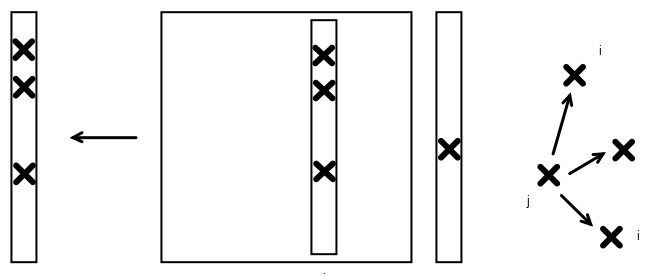
\includegraphics[scale=.5]{mvp-push}
  \caption{Push model of graph algorithms, depicted in matrix-vector form}
  \label{fig:mvp-push}
\end{figure}

In a picture, we see that we can call the algorithm we have just derived
a `push model',
since it repeatedly pushes the value of one node onto its neighbors.
This is analogous to one form of the matrix-vector product,
where the result vector is the sum of columns of the matrix.

While the algorithm is intuitive, as regards performance it is not great.
\begin{itemize}
\item Since the result vector is repeatedly updated, it is hard to cache it.
\item From nature of the push model, this variant is hard to parallelize,
  since it may involve conflicting updates.
  Thus a threaded code requires atomic operations, critical section, locks,
  or somesuch. A~distributed memory code is even harder to write.
\end{itemize}

\Level 2 {The `pull' model}

\begin{figure}[ht]
  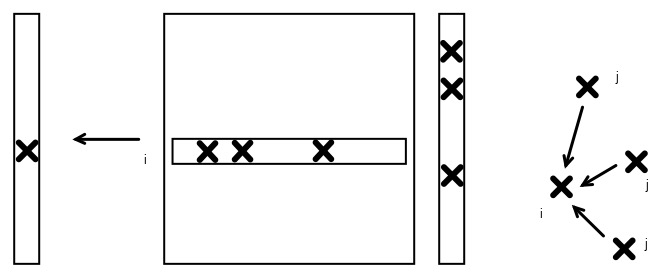
\includegraphics[scale=.5]{mvp-pull}
  \caption{Pull model of graph algorithms, depicted in matrix-vector form}
  \label{fig:mvp-pull}
\end{figure}

Leaving the original $i,j$ nesting of the loops,
we can not optimize the outer loop by removing certain iterations,
so we wind up with:

\begin{tabbing}
for \=all nodes $i$\\
\> for \=nodes $\{ j\colon j\rightarrow i\}$\\
\>\> $y_i \bigoplus a_{ij}\otimes x_j$\\
\end{tabbing}

This is similar to the traditional inner-product based matrix vector product,
but as a graph algorithm this variant is not often seen in the traditional literature.
We can describe this as a `pull model', since for each node~$i$ it pulls updates
from all its neighbors~$j$.

Regarding performance we can now state that:
\begin{itemize}
\item As a sequential algorithm, this can easily cache the output vector.
\item This algorithm is easily parallizable over the $i$ index;
  there are no conflicting writes.
\item A distributed algorithm is also straightforward, with the computation
  preceeded by a (neighbor) allgather of the input vector.
\item However, as a traditionally expressed graph algorithm it is wasteful,
  with many updates of each $y_j$ component.
\end{itemize}

\begin{comment}
%%%% move this to the ISP book as a project
\Level 1 {Sample implementation}

We assume that we have types \lstinline{vectorvalue} and \lstinline{matrixvalue}:
\begin{itemize}
\item
  vector values can take on a numerical value, or have a exceptional
  value \lstinline{undefined};
\item matrix values are \lstinline{empty}/\lstinline{filled}
  for \indextermsub{unweighted}{graph}s,
  or any numerical value for \indextermsub{weighted}{graph}s.
\end{itemize}

The most important part of the code is the matrix-vector multiplication;
we give the left multiplication since that is most common in graph computations.
%
\cxxverbatimsnippet{graphmultiply}
%
The multiplication routine takes two function pointers:
\begin{itemize}
\item a multiplication function for vector and matrix elements; and
\item an addition function for performing a reduction on vector elements.
\end{itemize}

We demonstrate this with two simple examples.
First we do a single matrix-vector multiplication,
with a matrix that connects each node to its successor
modulo the matrix size:
\[ m_{ij} = \delta_{i+1,j} \]
We apply this to a vector corresponding to a single vertex:
%
\snippetwithoutput{graphshift}{code/graph}{graph1}

In the second example we take the same matrix,
but now compute the single-source shortest path to each node.
This makes the multiplication and addition routines
marginally more complex:
%
\cxxverbatimsnippet{graphpathmultadd}

We now apply the matrix-vector multiplication
until we have found the distance to each vertex:
%
\snippetwithoutput{graphdistloop}{code/graph}{graph2}
\end{comment}

\Level 0 {`Real world' graphs}

In discussions such as in section~\ref{sec:2dbvp} you have seen how
the discretization of \acp{PDE} leads to computational problems that
has a graph aspect to them. Such graphs have properties that make them
amenable to certain kinds of problems.
%
For instance, using \acp{FDM} or \acp{FEM} to model two or
three-dimensional objects leads graphs where each node is connected to
just a few neighbours. This makes it easy to find
\indextermp{separator}, which in turn allows such solution methods as
\indexterm{nested dissection}; see section~\ref{sec:dissection}.

There are however applications with computationally intensive graph
problems that do not look like \ac{FEM} graphs. We will briefly look
at the example of the world-wide web, and algorithms such
\indexterm{Google}'s \indexterm{PageRank} which try to find
authoratative nodes.

For now, we will call such graphs \indextermsubp{random}{graph},
although this term has a technical meaning
too~\cite{Erdos:randomgraph}.

\Level 1 {Parallelization aspects}

In section~\ref{sec:pspmvp} we discussed the parallel evaluation
of the sparse matrix-vector product. Because of the sparsity, 
only a partitioning by block rows or columns made sense.
In effect, we let the partitioning be determined by one of the problem
variables. This is also the only strategy that makes sense for
single-source shortest path algorithms.

\begin{exercise}
  Can you make an \textit{a priori} argument for basing the
  parallelization on a distribution of the vector? How much data is
  involved in this operation, how much work, and how many sequential
  steps?
\end{exercise}

\Level 1 {Properties of random graphs}

The graphs we have seen in most of this course have properties that
stem from the fact that they model objects in our three-dimensional
world. Thus, the typical distance between two nodes is
typically~$O(N^{1/3})$ where $N$ is the number of nodes. Random graphs
do not behave like this: they often have a \indexterm{small world}
property where the typical distance is~$O(\log N)$. A~famous example
is the graph of film actors and their connection by having appeared in
the same movie: according to `Six degrees of separation', no two actors
have a distance more than six in this graph. In graph terms this means
that the diameter of the graph is six.

Small-world graphs have other properties, such as the existence of
cliques (although these feature too in higher order \ac{FEM} problems)
and hubs: nodes of a high degree. This leads to implications such as
the following: deleting a random node in such a graph does not have a
large effect on shortest paths.

\begin{exercise}
  Considering the graph of airports and the routes that exist between
  them. If there are only hubs and non-hubs, argue that deleting a
  non-hub has no effect on shortest paths between other airports. On
  the other hand, consider the nodes ordered in a two-dimensional
  grid, and delete an arbitrary node. How many shortest paths are affected?
\end{exercise}

\begin{notready}
\Level 1 {Concepts}

Two measures of centrality: eigenvector centrality and
betweenness. Low EC and high betweenness indicates a `gatekeeper'
function.

\begin{description}
  \item[Degree, diameter,distance] are defined as usual.
  \item[Betweenness]%\footnote{\url{http://en.wikipedia.org/wiki/Betweenness#Betweenness_centrality}}
    is defined as 
    \[ C(v)=\frac
       {\sum_{s\not=t\not=v} \#\hbox{shortest paths between $s,t$}}
       {\sum_{s\not=t\not=v} \#\hbox{shortest paths between $s,t$ that go through $v$}}
    \]
  \item[Eigenvector centrality] is the magnitude of a node's component
    in the Perron vector; see section~\ref{sec:pagerank}.
  \item[Closeness] measures the average distance of a node to all
    others:
    \[ c(v) = \frac{1}{n-1}\sum_{t\not=v}d(t,v). \]
  \item[Clustering coefficient] measures how much of a graph is
    organized in cliques. A~global coefficient is
    \[ \frac{\#\hbox{closed triplets}}{\#\hbox{open triplets}} \]
    where an open triplet is a triplet $i,j,k$ so that
    \[ (i,j)\in E,\quad (i,k)\in E, \quad (j,k)\not\in E \]
    while for a closed triplet the last relation is an
    inclusion. A~local definition is based on the fact that in a
    \indexterm{clique} of $k$ nodes there are $k(k-1)/2$ edges (in an
    undirected graph). Defining the \indexterm{neighbourhood} of a
    node~$i$ as 
    \[ N_i=\{j\not=i\colon (i,j)\in E\}, \]
    the local clustering coefficient can be defined as 
    \[ \frac{|\{e_{jk}\}_{j,k\in N_i}|}{k(k-1)/2}. \]
\end{description}
\end{notready}

\Level 0 {Hypertext algorithms}
\label{sec:pagerank}

There are several algorithms based on linear algebra
for measuring the importance of web
sites~\cite{Langville2005eigenvector}
and ranking \indextermsub{web}{search} results.
We will briefly define a few
and discuss computational implications.

\Level 1 {HITS}
\index{HITS|(}

In the HITS (Hypertext-Induced
Text Search) algorithm, sites have a \emph{hub} score that measures how many
other sites it points to, and an \emph{authority} score that measures
how many sites point to it. To calculate such scores we define an
\indexterm{incidence matrix}~$L$, where
\[ L_{ij}=
\begin{cases}
  1&\mbox{document $i$ points to document $j$}\\
  0&\mbox{otherwise}
\end{cases}
\]
The authority scores $x_i$ are defined as the sum of the hub scores
$y_j$ of everything that points to~$i$, and the other way around. Thus
\[
\begin{array}{l}
  x=L^ty\\ y=Lx
\end{array}
\]
or $x=LL^tx$ and $y=L^tLy$, showing that this is an eigenvalue
problem. The eigenvector we need has only nonnegative entries; this is
known as the \indexterm{Perron vector} for a
\indextermsub{nonnegative}{matrix}, see appendix~\ref{app:perron}. The
Perron vector is computed by a \indexterm{power method}; see
section~\ref{app:power-method}.

A practical search strategy is:
\begin{itemize}
\item Find all documents that contain the search terms;
\item Build the subgraph of these documents, and possible one or two
  levels of documents related to them;
\item Compute authority and hub scores on these documents, and present
  them to the user as an ordered list.
\end{itemize}

\index{HITS|)}

\Level 1 {PageRank}
\index{PageRank|(textbf}

The PageRank~\cite{PageBrin:PageRank} basic idea is similar to
HITS:
it models the question
`if the user keeps clicking on links that are somehow the
most desirable on a page, what will overall be the set of the most
desirable links'. 
This is modeled by defining
the ranking of a web page is the sum of the rank of all pages
that connect to it. The algorithm It is often phrased iteratively:
%
\begin{displayalgorithm}
  \While{Not converged}
        { \For { all pages $i$}
          {
            $\mathrm{rank}_i \leftarrow \epsilon +
            (1-\epsilon) \sum_{j\colon\mathrm{connected}j\rightarrow i}\mathrm{rank}_j$
          } \;
          normalize the ranks vector \;
        }
\end{displayalgorithm}
%
where the ranking is the fixed point of this algorithm.
The $\epsilon$ term solve the problem that if a page has
no outgoing links, a user that would wind up there would never
leave. 

\begin{exercise}
  Argue that this algorithm can be interpreted in two different ways,
  roughly corresponding to the Jacobi and Gauss-Seidel iterative
  methods; section~\ref{sec:jacobi-seidel}.
\end{exercise}

\begin{exercise}
  In the PageRank algorithm, each page `gives its rank' to the ones it
  connects to. Give pseudocode for this variant. Show that it
  corresponds to a matrix-vector product by columns, as opposed to by
  rows for the above formulation. What would be a problem implementing
  this in shared memory parallelism?
\end{exercise}

For an analysis of this method, including the question of whether it
converges at all, it is better to couch it completely in
linear algebra terms.
Again we define a connectivity matrix
\[ M_{ij}=
\begin{cases}
  1&\mbox{if page $j$ links to $i$}\\
  0&\mbox{otherwise}
\end{cases}
\]
With $e=(1,\ldots,1)$, the vector $d^t=e^tM$ counts how many links
there are on a page: $d_i$~is the number of links on page~$i$. We
construct a diagonal matrix $D=\diag(d_1,\ldots)$ we normalize $M$ to
$T=MD\inv$. 

Now the columns sums (that is, the sum of the elements in any column)
of $T$ are all~$1$, which we can express as $e^tT=e^t$ where
$e^t=(1,\ldots,1)$. Such a matrix is
called \indextermsub{stochastic}{matrix}. It has the following
interpretation:
\begin{quote}
  If $p$ is a \indexterm{probability vector}, that is, $p_i$ is the
  probability that the user is looking at page~$i$, then $Tp$ is the
  probability vector after the user has clicked on a random link.
\end{quote}

\begin{exercise}
  Mathematically, a probability vector is characterized by the fact
  that the sum of its elements is~1. Show that the product of a
  stochastic matrix and a probability vector is indeed again a
  probability vector.
\end{exercise}

The PageRank algorithm as formulated above
would correspond to taking an
arbitrary stochastic vector~$p$, computing the \indexterm{power method}
$Tp,T^2p,T^3p,\ldots$ and
seeing if that sequence converges to something.

There are few problems with this basic algorithm, such as
pages with no outgoing links. In general, mathematically we are
dealing with `invariant subspaces'. Consider for
instance an web with only 2 pages and the following
\indextermbus{adjacency}{matrix}:
\[ A=
\begin{pmatrix}
  1/2&0\\ 1/2&1
\end{pmatrix}.
\]
Check for yourself that this corresponds to the second page having no
outgoing links. Now let $p$ be the starting vector $p^t=(1,1)$, and
compute a few iterations of the power method. Do you see that the
probability of the user being on the second page goes up to~1? The
problem here is that we are dealing with a
\indextermsub{reducible}{matrix}.

To prevent this problem, PageRank
introduces another element: sometimes the user
will get bored from clicking, and will go to an arbitrary page (there
are also provisions for pages with no outgoing links). If we
call $s$ the chance that the user will click on a link, then the
chance of going to an arbitrary page is $1-s$. Together, we now have
the process
\[ p'\leftarrow sTp+(1-s)e, \]
that is, if $p$~is a vector of probabilities then $p'$ is a vector of
probabilities that describes where the user is after making one page
transition, either by clicking on a link or by `teleporting'.

The PageRank vector is the stationary point of this process; you can
think of it as the probability distribution after the user has made
infinitely many transitions. The PageRank vector satisfies
\[ p=sTp+(1-s)e \Leftrightarrow (I-sT)p=(1-s)e. \]
Thus, we now have to wonder whether $I-sT$ has an inverse.
If the inverse exists it satisfies
\[ (I-sT)\inv = I+sT+s^2T^2+\cdots \]
It is not hard to see that the inverse exists: with the Gershgorin theorem
(appendix~\ref{app:gershgorin}) you can see that the eigenvalues of
$T$ satisfy $|\lambda|\leq 1$. Now use that $s<1$, so the series of
partial sums converges.

The above formula for the inverse also indicates a way to compute the
PageRank vector~$p$ by using a series of matrix-vector
multiplications.

\begin{exercise}
  Write pseudo-code for computing the PageRank vector, given the
  matrix~$T$. Show that you never need to compute the powers of~$T$
  explicitly. (This is an instance of \indexterm{Horner's rule}).
\end{exercise}

In the case that $s=1$, meaning that we rule out teleportation, the
PageRank vector satisfies $p=Tp$, which is again the problem of
finding the \indexterm{Perron vector}; see appendix~\ref{app:perron}.

We find the Perron vector by a power iteration (section~\ref{app:power-method})
\[ p^{(i+1)} = T p^{(i)}. \]
This is a sparse matrix vector product, but unlike in the \ac{BVP}
case the sparsity is unlikely to have a structure such as
bandedness. Computationally, one probably has to use the same
parallelism arguments as for a dense matrix: the matrix has to be
distributed two-dimensionally~\cite{OgAi:sparsestorage}.

\index{PageRank|)}

\Level 0 {Large-scale computational graph theory}
\label{sec:random-graph-product}

In the preceding sections you have seen that many graph algorithms
have a computational structure that makes the matrix-vector product
their most important kernel. Since most graphs are of low degree 
relative to the number of nodes, the product is a \emph{sparse}
matrix-vector product.

While the dense matrix-vector product relies on collectives
(see section~\ref{sec:parallel-dense-mvp}),
the sparse case uses point-to-point communication, that is,
every processor sends to just a few neighbors, and receives
from just a few.
This makes sense for the type of sparse matrices
that come from \acp{PDE}
which have a clear structure, as you saw 
in section~\ref{sec:2dbvp}. However, there are 
sparse matrices that are so random that you essentially
have to use dense techniques; see
section~\ref{sec:random-graph-product}.

In many cases we can then, as in section~\ref{sec:pspmvp},
make a one-dimensional distribution of the matrix,
induced by a distribution of the graph nodes: if a processor
owns a graph node~$i$, it owns all the edges~$i,j$.

However, often the computation is very unbalanced. For instance,
in the single-source shortest path algorithm only the vertices
along the front are active. For this reason, sometimes a distribution
of edges rather than vertices makes sense. For an even balancing
of the load even random distributions can be used.

The \indextermsub{parallelization of the}{Floyd-Warshall algorithm}
(section~\ref{sec:floyd}) proceeds along different lines. Here we don't
compute a quantity per node, but a quantity that is a function of pairs
of nodes, that is, a matrix-like quantity. Thus, instead of distributing
the nodes, we distribute the pair distances.

\Level 1 {Distribution of nodes vs edges}

Sometimes we need to go beyond a one-dimensional decomposition in dealing
with sparse graph matrices.
Let's assume that we're dealing with a graph that has a structure that
is more or less random, for instance in the sense that the chance of
there being an edge is the same for any pair of vertices. Also
assuming that we have a large number of vertices and edges, every
processor will then store a certain number of vertices. The conclusion
is then that the chance that any pair of processors needs to exchange
a message is the same, so the number of messages is~$O(P)$. (Another
way of visualizing this is to see that nonzeros are randomly
distributed through the matrix.) This does not give a scalable
algorithm.

The way out is to treat this sparse matrix as a dense one, and invoke
the arguments from section~\ref{sec:densescaling} to decide on a
two-dimensional distribution of the matrix.
(See~\cite{Yoo:2005:scalable-bfs} for an application to the \ac{BFS}
problem; they formulate their algorithm in graph terms, but the
structure of the 2D matrix-vector product is clearly recognizable.)
The two-dimensional product algorithm only needs collectives in
processor rows and columns, so the number of processors involved
is~$O(\sqrt P)$.

\Level 1 {Hyper-sparse data structures}

With a two-dimensional distribution of sparse matrices,
it is conceivable that some processes wind up with matrices
that have empty rows. Formally, a matrix is called
\emph{hyper-sparse}\index{sparse!matrix!hyper-sparse}
if the number of nonzeros is (asymptotically) less than the dimension.

In this case, \ac{CRS} format can be inefficient,
and something called
\emph{double-compressed storage}\index{sparse!matrix!doubly-compressed}
can be used~\cite{BulucGilbert:hypersparse}.

\endinput

Triadic closure: if $(i,j)\in E$ and $(i,k)\in E$ then $(j,k)\in E$;
example: friend or trust relationship.

A \indextermsub{scale-free}{network}, or one that observes a
\indexterm{power law}, is one where the fraction of nodes with
degree~$k$ is proportional to $k^{-\gamma}$ where $\gamma$ is
positive, typically $2<\gamma<3$. There are claims that graphs such as
the \ac{WWW} obey power laws; this is a claim about the logical
structure, not the physical one, which is very hard to
infer~\cite{Willinger:internet}.

A small-world network can be created by extending an existing network
by \emph{preferential attachment}:
the chance of attaching a new node is proportional to the degree
of the old node.

Power law networks usually have a very small diameter.

